\documentclass[aspectratio=169,11pt]{beamer}

\usepackage{graphicx}
\usepackage{tikz}
\usetikzlibrary{positioning,arrows.meta}
\usepackage{xcolor}
\usepackage{booktabs}
\usepackage{tabularx}
\usepackage{array}
\usepackage{ragged2e}

\definecolor{GEUBlue}{RGB}{20,55,105}
\definecolor{GEULightBlue}{RGB}{238,244,251}
\definecolor{GEUGrey}{RGB}{90,90,90}
\definecolor{GEULightGrey}{RGB}{245,246,248}

\usetheme{default}
\setbeamertemplate{navigation symbols}{}
\setbeamertemplate{blocks}[rounded][shadow=false]
\setbeamercolor{normal text}{fg=black,bg=white}
\setbeamercolor{frametitle}{fg=GEUBlue}
\setbeamercolor{structure}{fg=GEUBlue}
\setbeamercolor{block title}{fg=GEUBlue,bg=GEULightBlue}
\setbeamercolor{block body}{fg=black,bg=GEULightBlue}
\setbeamerfont{frametitle}{size=\Large,series=\bfseries}

% Replace with the actual logo filename
\newcommand{\GEULogo}{logo.jpeg}

% Header and footer
\setbeamertemplate{headline}{%
  \begin{tikzpicture}[remember picture,overlay]
    \node[anchor=north east,xshift=-0.30cm,yshift=-0.12cm]
      at (current page.north east)
      {\includegraphics[height=0.62cm]{\GEULogo}};
  \end{tikzpicture}
  \vspace{0.72cm}
}
\setbeamertemplate{frametitle}{%
  \vspace{0.03cm}
  \insertframetitle\par
  \vspace{0.04cm}
  \textcolor{GEUBlue}{\rule{\textwidth}{0.9pt}}
  \vspace{0.03cm}
}
\setbeamertemplate{footline}{%
  \leavevmode
  \hbox{%
  \begin{beamercolorbox}[wd=.82\paperwidth,ht=0.32cm,dp=0.10cm,leftskip=.3cm]{author in head/foot}
    \tiny Department of Computer Science \& Engineering | Graphic Era (Deemed to be University)
  \end{beamercolorbox}%
  \begin{beamercolorbox}[wd=.18\paperwidth,ht=0.32cm,dp=0.10cm,rightskip=.3cm]{date in head/foot}
    \hfill\tiny\insertframenumber/\inserttotalframenumber
  \end{beamercolorbox}}
}

\newcommand{\smallnote}[1]{\vspace{0.08cm}{\scriptsize\color{GEUGrey}#1}}
\newcommand{\placeholder}[1]{\textit{\color{GEUGrey}#1}}

\title{\textbf{Project-Based Learning}\\[2mm]\large Phase-I Evaluation}
\author{\textbf{RideSync: A Graph-Based Smart Cab Booking and Dispatch Simulation System}\\Team ID: DSCPP-III-2026-T151}
\institute{Department of Computer Science \& Engineering\\Graphic Era (Deemed to be University), Dehradun}
\date{Academic Session 2026--27}

\begin{document}

% 1
\begin{frame}[plain]
\begin{tikzpicture}[remember picture,overlay]
\draw[GEUBlue,line width=3pt] (current page.north west) -- (current page.north east);
\node[anchor=north east,xshift=-0.45cm,yshift=-0.35cm] at (current page.north east)
{\includegraphics[height=1.0cm]{\GEULogo}};
\node[align=center,text width=.84\paperwidth] at ([yshift=.25cm]current page.center)
{{\color{GEUBlue}\fontsize{26}{30}\selectfont\bfseries PROJECT-BASED LEARNING}\\[3mm]
 {\fontsize{18}{22}\selectfont PHASE-I EVALUATION}\\[7mm]
 {\color{GEUGrey}\Large\bfseries RideSync: A Graph-Based Smart Cab Booking and Dispatch Simulation System}\\[3mm]
 {\color{GEUBlue}\normalsize Team ID: DSCPP-III-2026-T151}};
\node[align=center,anchor=south,yshift=.42cm] at (current page.south)
{\bfseries Department of Computer Science \& Engineering\\
Graphic Era (Deemed to be University), Dehradun\\[-1mm]
\scriptsize Academic Session 2026--27};
\end{tikzpicture}
\end{frame}

% 2
\begin{frame}{Team \& Mentor Details}

\begin{columns}[T,totalwidth=\textwidth]

\column{.48\textwidth}

\begin{block}{Team Information}
\begin{tabular}{@{}p{2.5cm}p{4.2cm}@{}}
\textbf{Team ID:} & DSCPP-III-2026-T151\\
\textbf{Semester:} & 3rd\\
\textbf{Team Name:} & The Four Bytes\\
\textbf{Domain:} & Data Structures \&\\
& Programming in C++
\end{tabular}
\end{block}


\column{.48\textwidth}

\begin{block}{Team Members}
1.\quad Gupta, Tanvi -- 2510010362 (Team Lead)\\
2.\quad Jahnavi -- 2510380066\\
3.\quad Tyagi, Nishtha -- 2510370096\\
4.\quad Sharma, Dhairya -- 2510011490
\end{block}

\end{columns}

\vspace{2mm}

\begin{block}{Mentor}
\placeholder{Mentor: Dr. Hemant Singh Pokhariya}
\hfill
\textbf{Interactions completed:3}
\end{block}

\end{frame}
% 3
\begin{frame}{Problem Statement \& Motivation}

\vspace{-6mm}

\begin{block}{Problem Statement}
\small
Traditional cab booking through phone calls or taxi stands is inefficient and unorganised. Manual driver assignment ignores distance and availability, while the lack of shortest-path calculation can increase waiting time and lead to inconsistent fares.
\end{block}

\vspace{1mm}

\begin{columns}[T,totalwidth=\textwidth]

\column{.48\textwidth}
\textbf{\color{GEUBlue}Motivation}
\begin{itemize}\itemsep1.5pt
\item Traditional booking lacks efficiency
\item No shortest-path calculation
\item Manual, non-optimal driver assignment
\item Use OOP, weighted graphs, Dijkstra's Algorithm, and a priority queue for efficient booking
\end{itemize}

\column{.48\textwidth}
\textbf{\color{GEUBlue}Target Users / Stakeholders}
\begin{itemize}\itemsep1.5pt
\item Customers booking cabs
\item Drivers assigned rides
\item Admin / system manager
\end{itemize}

\end{columns}

\end{frame}
% 4
\begin{frame}{Objectives}

\small
\textbf{\color{GEUBlue}Project Objectives}
\vspace{1mm}

\begin{enumerate}\itemsep1.5pt
\item Design a modular, console-based Cab Booking System in C++17
\item Build well-encapsulated Customer, Driver, Admin, and Booking modules
\item Represent city locations and roads as a weighted graph and compute shortest routes using Dijkstra's Algorithm
\item Assign the most suitable available driver using a priority queue
\item Estimate fares based on the computed route distance
\item Persist customer, driver, cab, and booking data using file handling
\end{enumerate}

\vspace{1mm}

\begin{center}
\colorbox{GEULightBlue}{%
\parbox{0.80\textwidth}{%
\centering
\small
\textbf{Key Objective:} Design and implement a modular, console-based Cab Booking System in C++17 that demonstrates Object-Oriented Programming and core Data Structures and Algorithms.%
}}
\end{center}

\end{frame}

% 5
\begin{frame}{Proposed Solution}

\small

\vspace{-4mm}

\begin{columns}[T,totalwidth=\textwidth]

\column{.48\textwidth}

\textbf{\color{GEUBlue}Proposed Approach}
\begin{enumerate}\itemsep1pt
\item Enter pickup and drop locations
\item Represent locations and roads as a weighted graph
\item Find shortest route using Dijkstra's Algorithm
\item Select the best driver using a priority queue
\item Calculate fare from route distance
\item Store booking data using file handling
\item Display booking result and history
\end{enumerate}

\column{.48\textwidth}

\textbf{\color{GEUBlue}Key Features}
\begin{itemize}\itemsep1.5pt
\item Customer registration/login and cab booking
\item Driver registration/login and availability management
\item Admin management of cabs and drivers
\item Graph-based shortest-route calculation
\item Priority-queue-based driver assignment
\item Distance-based fare calculation
\item Booking history and cancellation handling
\end{itemize}

\end{columns}

\vspace{1mm}


\end{frame}

% 6
\begin{frame}{Integration of PBL Course Concepts}
\scriptsize
\begin{center}
\renewcommand{\arraystretch}{1.25}
\begin{tabularx}{.96\textwidth}{@{}>{\bfseries}p{4.0cm}X p{2.4cm}@{}}
\toprule
Course/Area & Concepts Applied & Project Module\\
\midrule
Data Structures \& Algorithms & Graph, Priority Queue, Stack, Linked List, Dijkstra's Algorithm, Searching, Sorting & Routing, Driver Assignment \& Booking History\\
OOP with C++ & Classes \& Objects, Constructors, Inheritance, Virtual Functions, Polymorphism, Encapsulation, STL, File Handling & Customer, Driver, Cab, Admin \& Booking\\
\bottomrule
\end{tabularx}
\end{center}

\vfill

\begin{center}
\colorbox{GEULightBlue}{\parbox{.86\textwidth}{\centering
\textbf{Requirement:} Demonstrate meaningful integration of Data Structures \& Algorithms and OOP with C++ in \textbf{one} project.}}
\end{center}
\end{frame}

% 7
\begin{frame}{System Architecture / Workflow}

\vspace{-3mm}

\begin{center}
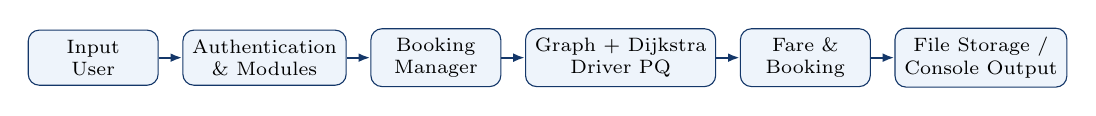
\begin{tikzpicture}[
node distance=3mm,
box/.style={
rectangle,
rounded corners,
draw=GEUBlue,
fill=GEULightBlue,
minimum width=1.65cm,
minimum height=7mm,
align=center,
font=\scriptsize
},
arrow/.style={
-{Latex[length=1.5mm]},
thick,
draw=GEUBlue
}
]

\node[box] (a) {Input\\User};
\node[box,right=of a] (b) {Authentication\\\& Modules};
\node[box,right=of b] (c) {Booking\\Manager};
\node[box,right=of c] (d) {Graph + Dijkstra\\Driver PQ};
\node[box,right=of d] (e) {Fare \&\\Booking};
\node[box,right=of e] (f) {File Storage /\\Console Output};

\draw[arrow] (a)--(b);
\draw[arrow] (b)--(c);
\draw[arrow] (c)--(d);
\draw[arrow] (d)--(e);
\draw[arrow] (e)--(f);

\end{tikzpicture}
\end{center}

\vspace{1mm}

\begin{columns}[T,totalwidth=\textwidth]

\column{.48\textwidth}

\textbf{\color{GEUBlue}Major Components}
\begin{itemize}\itemsep1pt
\item Customer, Driver, Cab, Admin classes
\item Authentication Manager \& Booking Manager
\item Weighted graph with Dijkstra's Algorithm and driver priority queue
\end{itemize}

\column{.48\textwidth}

\textbf{\color{GEUBlue}Data / Control Flow}
\begin{itemize}\itemsep1pt
\item User logs in and selects a role (Customer/Driver/Admin)
\item Booking Manager computes route, assigns driver, calculates fare
\item Results and records stored via file handling and shown on console
\end{itemize}

\end{columns}

\end{frame}
% 8
\begin{frame}{Technology Stack \& Methodology}

\small

\vspace{-3mm}

\begin{columns}[T,totalwidth=\textwidth]

\column{.55\textwidth}

\begin{block}{Technology Stack}
\footnotesize
\begin{itemize}\itemsep1pt
\item Programming Language: C++17
\item STL: vector, queue, priority\_queue, unordered\_map, stack
\item OOP: Classes \& Objects, Encapsulation, Inheritance
\item Data Structures: Graph, Linked List, Stack, Queue
\item Algorithms: Dijkstra's Algorithm, Searching, Sorting
\item Persistence: fstream / flat text files
\item IDE: VS Code
\item Version Control: GitHub
\end{itemize}
\end{block}

\column{.41\textwidth}

\begin{block}{Development Methodology}
\begin{enumerate}\itemsep1pt
\item Problem Definition
\item Requirement Analysis
\item System Design
\item Module/Class Design
\item Implementation
\item Integration
\item Testing \& Debugging
\item Documentation / Demonstration
\end{enumerate}
\end{block}

\end{columns}

\vspace{1mm}

\begin{center}
\footnotesize

\end{center}

\end{frame}

% 9
\begin{frame}{Initial Progress \& Team Contribution}

\begin{columns}[T,totalwidth=\textwidth]

\column{.43\textwidth}

\textbf{\color{GEUBlue}Progress Achieved}
\begin{itemize}\itemsep2pt
\item Problem definition and requirement analysis completed
\item Overall system design and approach finalized
\item System architecture planned
\item Modules identified
\item Algorithms and data structures identified
\item Technology stack selected
\end{itemize}

\column{.55\textwidth}

\textbf{\color{GEUBlue}Individual Contribution}

\vspace{2mm}

\small
\begin{tabular}{|c|p{2.5cm}|p{2.9cm}|}
\hline
\textbf{Member} & \textbf{Role} & \textbf{Contribution} \\
\hline
Tanvi & Team Lead & Booking Module \\
\hline
Nishtha & Developer & Booking Module \\
\hline
Jahnavi & Developer/Docs & Graph \& Dijkstra \\
\hline
Dhairya & DB/Testing & Priority Queue \& Testing \\
\hline
\end{tabular}

\end{columns}

\end{frame}

% 10
\begin{frame}{Roadmap, Expected Outcomes \& References}

\scriptsize
\vspace{-5mm}

\begin{columns}[T,totalwidth=\textwidth]

%------------------------------------------------
% LEFT COLUMN
%------------------------------------------------
\column{.64\textwidth}

\textbf{\color{GEUBlue}Roadmap}

\begin{enumerate}
\setlength{\itemsep}{1pt}
\setlength{\parskip}{0pt}
\item Phase 1 (Wk 1--2): Requirements \& system design
\item Phase 2 (Wk 3--4): Classes, authentication \& user modules
\item Phase 3 (Wk 5--6): Graph, Dijkstra's Algorithm \& driver assignment
\item Phase 4 (Wk 7--8): Booking, fare calculation \& persistence
\item Phase 5 (Wk 9--10): Integration, testing \& demo
\end{enumerate}

\vspace{1 mm}

\textbf{\color{GEUBlue}Expected Outcomes}

\begin{itemize}
\setlength{\itemsep}{1pt}
\setlength{\parskip}{0pt}
\item Working console-based Cab Booking System
\item Customer, Driver \& Admin modules
\item Dijkstra-based routing \& driver assignment
\item Fare calculation, booking history \& cancellation
\item File-based data persistence
\end{itemize}

%------------------------------------------------
% RIGHT COLUMN
%------------------------------------------------
\column{.34\textwidth}

\textbf{\color{GEUBlue}References}

\begin{enumerate}
\setlength{\itemsep}{1pt}
\setlength{\parskip}{0pt}
\item cppreference.com -- C++17 Library
\item GeeksforGeeks -- OOP in C++
\item GeeksforGeeks -- Dijkstra's Algorithm
\item cplusplus.com -- STL Containers
\item cplusplus.com -- File Handling
\end{enumerate}

\vspace{3mm}

\begin{center}
\colorbox{GEUBlue}{%
\parbox{.98\linewidth}{%
\centering
\color{white}
\textbf{Thank You}\\[-1pt]
Questions \& Suggestions
}}
\end{center}

\end{columns}

\end{frame}
\end{document}